\باب{توانائی اور برقی دباو}

\حصہ{توانائی اور کام}
قوت \عددیء{F} کی سمت میں فاصلہ \عددیء{\dif L} طے کرنے سے 
\begin{align*}
\dif W= F \dif L
\end{align*}
\اصطلاح{کام} کیا جاتا ہے۔اگر قوت اور طے کردہ فاصلہ ایک ہی سمت میں نہ ہوں تب  قوت کا وہ حصہ جو طے کردہ فاصلے کی سمت میں ہو اور طے شدہ فاصلے  کے حاصل ضرب کو \اصطلاح{کام}\فرہنگ{کام}\حاشیہب{work}\فرہنگ{work} کہتے ہیں۔شکل \حوالہ{شکل_دباو_کام_کی_تعریف} کو دیکھتے ہوئے سمتیات کے استعمال سے 
\begin{align*}
\dif W&=F \cos \alpha  \dif L\\
&=\kvec{F} \cdot \dif \kvec{L}
\end{align*}
لکھا جا سکتا ہے جہاں \عددیء{F \cos \alpha \dif L} کو نقطہ ضرب کی مدد سے \عددیء{\kvec{F} \cdot \dif \kvec{L}} لکھا گیا ہے۔
\begin{figure}
\centering
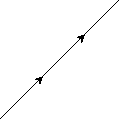
\includegraphics{figVoltageWork}
\caption{طے فاصلہ اور فاصلے کی سمت میں قوت کا حاصل ضرب کام کہلاتا ہے}
\label{شکل_دباو_کام_کی_تعریف}
\end{figure}

زمین اور کمیت \عددیء{m} کے درمیان قوت ثقل \عددیء{\kvec{F}_G=-\tfrac{GMm}{r^2}\ar} پایا جاتا ہے\حاشیہد{\عددیء{\ar}  اکائی سمتیہ ہے۔} جس میں \عددیء{\tfrac{GM}{r^2}=g} لکھتے ہوئے  \عددیء{\kvec{F}_G=-mg \ar} لکھا جا سکتا ہے۔کام کرتے ہوئے کمیت کو \عددیء{\Delta h \ar} اونچائی پر منتقل کرنے  کی خاطر قوت ثقل کے خلاف
\begin{align*}
\kvec{F}_{\textrm{لاگو}}=-\kvec{F}_G
\end{align*}
لاگو کرتے ہوئے
\begin{align*}
\Delta W=\kvec{F}_{\textrm{لاگو}} \cdot \Delta h \ar=mg \Delta h
\end{align*}
 توانائی درکار ہو گی۔کام کرنے کے لئے درکار توانائی کمیت میں منتقل ہو جاتی ہے جسے \اصطلاح{مخففی توانائی}\فرہنگ{مخفففی توانائی}\حاشیہب{potential energy}\فرہنگ{potential energy} کہتے ہیں۔اگر \عددیء{\Delta h} کی قیمت  \عددیء{r} کی نسبت سے  بہت کم نہ ہو تب \عددیء{g} کو مستقل تصور کرنا ممکن نہ ہو گا اور مخففی توانائی تکملہ کے ذریعہ حاصل کی جائے گی۔
\begin{align*}
W =-\int_{\textrm{ابتدا}}^{\textrm{اختتام}} \kvec{F}_G \cdot \dif \kvec{r}=\int_{\textrm{ابتدا}}^{\textrm{اختتام}} \frac{GMm }{r^2} dr
\end{align*}
ثقلی میدان میں کمیت کو ابتدائی نقطے سے اختتامی نقطے تک پہنچاتے ہوئے کوئی بھی راستہ اختیار کیا جا سکتا ہے۔اختیار کردہ راستے کا مخففی توانائی پر کسی قسم کا کوئی اثر نہیں ہوتا۔ایسے میدان جن میں دو نقطوں کے مابین مخفففی توانائی کا دارومدار، ابتدائی نقطے سے اختتامی نقطے تک پہنچنے کے راستے،  پر نہیں ہوتا \اصطلاح{قائم میدان}\فرہنگ{قائم میدان}\حاشیہب{conservative field}\فرہنگ{conservative field} کہلاتے ہیں۔ 

برقی میدان میں چارجوں کے حرکت کے مسئلے کو بھی اسی طرح حل کیا جاتا ہے۔برقی میدان \سمتیہ{E} میں چارج \عددیء{q} پر قوت \عددیء{\kvec{F}_E=q \kvec{E}} عمل کرتا ہے۔چارج کو فاصلہ \عددیء{\dif \kvec{L}} ہلانے کی خاطر اس قوت کے خلاف بیرونی
\begin{align*}
\kvec{F}_{\textrm{لاگو}} = -\kvec{F}_E
\end{align*}
قوت لاگو کرتے ہوئے
\begin{align}\label{مساوات_دباو_کام_کی_تعریف}
\dif W=-q \kvec{E} \cdot \dif \kvec{L}
\end{align}
کام\حاشیہب{work} کیا جاتا ہے۔کسی بھی ابتدائی نقطے سے اختتامی نقطے تک یوں
\begin{align}\label{مساوات_دباو_لکیری_تکملہ}
W=-q \int_{\textrm{ابتدا}}^{\textrm{اختتام}} \kvec{E} \cdot \dif\kvec{L}
\end{align}
توانائی درکار ہو گی۔

\حصہ{لکیری تکملہ}\حاشیہط{مکمل کرنا درکار ہے۔}
مساوات \حوالہ{مساوات_دباو_لکیری_تکملہ} لکیری تکملہ ہے جس پر مزید غور کرتے ہیں۔شکل \حوالہ{شکل_دباو_تکملہ_بمع_مجموعہ} میں \اصطلاح{یکساں}\فرہنگ{یکساں}\حاشیہب{uniform}\فرہنگ{uniform} اور وقت کے ساتھ نہ تبدیل ہونے والے میدان  \عددیء{\kvec{E}} میں  نقطہ \عددیء{O} سے نقطہ \عددیء{N} تک  چارج  کی منتقلی دکھائی گئی ہے۔یکساں میدان سے مراد ایسا میدان ہے جس میں \عددیء{\kvec{E}}  کی قیمت جگہ جگہ تبدیل نہیں ہوتی بلکہ اس کی قیمت ہر جگہ یکساں ہوتی ہے۔اسی طرح وقت کے ساتھ تبدیل ہوتے میدان کو  وقت کے ساتھ تغیر پذیر میدان کہا جائے گا۔یکساں میدان وقت کے ساتھ غیر تغیر پذیر میدان ہے۔

\begin{figure}
\centering
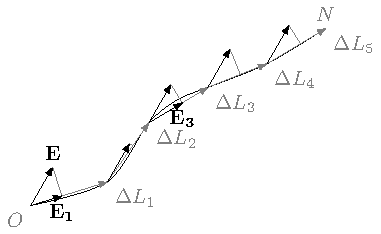
\includegraphics{figVoltageLineIntegralAsSum}
\caption{تکملہ دراصل چھوٹے حصوں کا مجموعہ ہوتا ہے۔}
\label{شکل_دباو_تکملہ_بمع_مجموعہ}
\end{figure}
شکل \حوالہ{شکل_دباو_تکملہ_بمع_مجموعہ} میں پورے راستے کو چھوٹے چھوٹے  ٹکڑے \عددیء{\Delta \kvec{L}_1}، \عددیء{\Delta \kvec{L}_2}، \عددیء{\cdots} میں تقسیم  کرتے ہوئے ایک ایک ٹکڑے پر حرکت کے لئے درکار توانائی مساوات \حوالہ{مساوات_دباو_کام_کی_تعریف} کی مدد سے  حاصل کی جا سکتی ہے۔یوں  \عددیء{\Delta \kvec{L}_1}  کے ابتدائی نقطے سے اختتامی نقطے تک چارج \عددیء{q} منتقل کرنے کی
 خاطر \عددیء{\Delta W=-q \kvec{E} \cdot \Delta \kvec{L}_1} توانائی درکار ہو گی۔یہی عمل راستے کے بقایا ٹکڑوں پر بھی لاگو کرتے ہوئے کُل درکار توانائی
\begin{gather}
\begin{aligned}\label{مساوات_دباو_مجموعہ_ٹکڑے}
W&=-q \kvec{E} \cdot \Delta \kvec{L}_1 -q \kvec{E} \cdot \Delta \kvec{L}_2 -q \kvec{E} \cdot \Delta \kvec{L}_3 -q \kvec{E} \cdot \Delta \kvec{L}_4 -q \kvec{E} \cdot \Delta \kvec{L}_5\\
&=-q \kvec{E} \cdot \left(\Delta \kvec{L}_1  +\Delta \kvec{L}_2 +\Delta \kvec{L}_3+\Delta \kvec{L}_4+\Delta \kvec{L}_5\right)
\end{aligned}
\end{gather}
لکھی جا سکتی ہے۔قوسین میں بند \عددیء{\Delta \kvec{L}_1  +\Delta \kvec{L}_2 +\Delta \kvec{L}_3+\Delta \kvec{L}_4+\Delta \kvec{L}_5} درحقیقت نقطہ \عددیء{O} سے \عددیء{N} تک کا  کُل سمتی راستہ \عددیء{\kvec{L}_{ON}} ہے۔یوں مندرجہ بالا مساوات کو
\begin{align}
W=-q \kvec{E} \cdot \kvec{L}_{ON}
\end{align}
لکھا جا سکتا ہے۔اگر شکل \حوالہ{شکل_دباو_تکملہ_بمع_مجموعہ} میں منتقلی کے راستے کے نہایت چھوٹے چھوٹے ٹکڑے \عددیء{\dif \kvec{L}} بنائے جائیں تو مساوات \حوالہ{مساوات_دباو_مجموعہ_ٹکڑے} کو تکمل کی شکل میں یوں لکھا جا سکتا ہے۔
\begin{align}
W=\int_O^N -q \kvec{E} \cdot \dif \kvec{L}
\end{align}
چونکہ \عددیء{q} اور \عددیء{\kvec{E}} کی قیمتیں مستقل ہیں  لہٰذا انہیں تکمل کے باہر لکھا جا سکتا ہے۔ایسا کرتے ہوئے
\begin{gather}
\begin{aligned}
W&=-q \kvec{E} \cdot  \int_O^N \dif \kvec{L}\\
&=-q \kvec{E} \cdot \kvec{L}_{ON}
\end{aligned}
\end{gather}
حاصل ہوتا ہے۔اس جواب سے ہم دیکھتے ہیں کہ درکار توانائی کا دارومدار \عددیء{q}، \عددیء{\kvec{E}} اور \عددیء{\kvec{L}_{ON}} پر ہے جہاں \عددیء{\kvec{L}_{ON}} نقطہ \عددیء{O} سے نقطہ \عددیء{N} تک سیدھی کھینچی لکیر ہے۔درکار توانائی کا اس سے کسی قسم کا کوئی تعلق نہیں کہ ابتدائی نقطے سے اختتامی نقطے جاتے ہوئے کون سا راستہ اختیار کیا گیا۔جیسا کہ پہلے ذکر کیا گیا، ایسے میدان کو \اصطلاح{قدامت پسند} میدان کہتے ہیں۔ہم جلد دیکھیں گے کہ غیر یکساں برقی میدان بھی قدامت پسند میدان ہوتا ہے البتہ تغیر پذیر  برقی میدان غیر قدامت پسند ہو سکتا ہے۔

\ابتدا{مثال}\شناخت{مثال_توانائی_سیدھی_لکیر_غیر_ہموار_میدان}
غیر یکساں، غیر تغیر پذیر میدان
\begin{align*}
\kvec{E}=(y+z)\ax+(x+z)\ay+(x+y)\az \quad \si{\volt \per \meter}
\end{align*}
میں \عددیء{N_1(1,0,2)} سے \عددیء{N_2(0,1,2)} تک سیدھی لکیر پر \عددیء{\SI{0.1}{\coulomb}} کا چارج منتقل کرنے کے لئے درکار توانائی حاصل  کریں۔ 
\begin{figure}
\centering
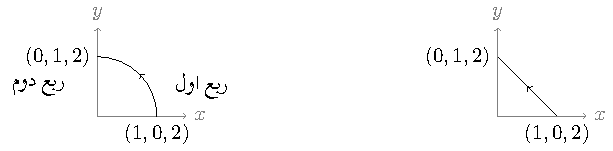
\includegraphics{figVoltageNonUniformNonTimeVaryingStraightLine}
\caption{چارج منتقل کرنے کے دو راستے۔}
\label{شکل_توانائی_چارج_منتقل_سیدھی_لکیر_گول_دائرہ}
\end{figure}

حل: شکل \حوالہ{شکل_توانائی_چارج_منتقل_سیدھی_لکیر_گول_دائرہ} میں چارج منتقل کرنے کا سیدھا راستہ دکھایا گیا ہے۔پہلے اس سیدھی لکیر کا مساوات حاصل کرتے ہیں۔اس لکیر کا ڈھلوان\حاشیہب{slope}
\begin{align*}
\textup{ڈھلوان}=m=\frac{y_2-y_1}{x_2-x_1}=\frac{1-0}{0-1}=-1
\end{align*}
 ہے لہٰذا سیدھی لکیر کی مساوات \عددیء{y=mx +c} میں نقطہ \عددیء{N_1} پُر کرتے ہوئے  \عددیء{0=-1 \times 1 +c} سے \عددیء{c=1} حاصل ہوتا ہے۔یوں لکیر کی مساوات
\begin{align}\label{مساوات_توانائی_سیدھی_لکیر_کی_مثال}
y=-x+1
\end{align}
ہے۔کارتیسی محدد میں کسی بھی راستے پر حرکت کرتے ہوئے 
\begin{align}
\dif \kvec{L}=\dif x \ax+\dif y \ay+\dif z \az
\end{align}
لکھا جاتا ہے۔یوں مساوات \حوالہ{مساوات_دباو_لکیری_تکملہ} سے حاصل ہو گا۔
\begin{align*}
W&=-q \int_{\textrm{ابتدا}}^{\textrm{اختتام}} \kvec{E} \cdot \dif\kvec{L}\\
&=-0.1 \int_{N_1}^{N_2} \left[ (y+z)\ax+(x+z)\ay+(x+y)\az \right] \cdot (\dif x \ax+\dif y \ay+\dif z \az)\\
&=-0.1 \int_{1}^{0} (y+z) \dif x -0.1 \int_{0}^{1}(x+z) \dif y-0.1 \int_{2}^{2} (x+y) \dif z
\end{align*}
آخری قدم پر تکمل کو تین حصوں میں لکھا گیا ہے جہاں پہلے حصے میں تکمل کو \عددیء{x} کے ساتھ حاصل کیا گیا ہے جبکہ دوسرے حصے میں تکمل کو \عددیء{y} کے ساتھ اور آخری حصے میں اسے \عددیء{z} کے ساتھ حاصل کیا گیا ہے۔پہلے حصے میں \عددیء{(y+z)} کا تکمل \عددیء{x} کے ساتھ ہے لہٰذا  \عددیء{(y+z)} کو \عددیء{x} کی صورت میں لکھنا ہو گا۔منتقلی کے راستے  پر \عددیء{z=2} ہے جبکہ  مساوات \حوالہ{مساوات_توانائی_سیدھی_لکیر_کی_مثال} میں \عددیء{y} کو \عددیء{x} کی صورت میں لکھا گیا ہے۔یوں پہلا تکمل
\begin{align*}
-0.1 \int_{1}^{0} [y+z]\dif x &=-0.1 \int_{1}^{0} [(-x+1)+2] \dif x\\
&=-0.1\left.\left(\frac{-x^2}{2}+3x\right) \right|_{1}^{0}\\
&=\SI{0.25}{\joule}
\end{align*}
یعنی جاول کے ایک چوتھائی کے برابر حاصل ہوتا ہے۔دوسرا تکمل \عددیء{y} کے ساتھ ہے لہٰذا تمام متغیرات  \عددیء{y} کی صورت میں لکھنے ہوں گے۔سیدھی لکیر کے مساوات سے  \عددی{x=-y+1} لکھا جا سکتا ہے جبکہ  پورے راستے پر \عددیء{z=2}  کے برابر ہے لہٰذا
\begin{align*}
-0.1 \int_{0}^{1} [x+z]\dif y &=-0.1 \int_{0}^{1} [(-y+1)+2] \dif y\\
&=-0.1 \left.\left(\frac{-y^2}{2}+3y\right) \right|_{0}^{1}\\
&=\SI{-0.25}{\joule}
\end{align*}
ہو گا۔تیسرے تکمل میں ابتدائی اور اختتامی نقطے ایک ہی ہیں لہٰذا یہ تکمل صفر کے برابر ہے۔ 
\begin{align*}
-0.1 \int_{2}^{2} (x+y) \dif z &=\SI{0}{\joule}
\end{align*}
اس طرح کُل درکار توانائی تینوں جوابات کا مجموعہ یعنی  \عددیء{\SI{0}{\joule}} ہو گی۔مثبت جواب کا مطلب یہ ہے کہ چارج کو منتقل کرنے کی خاطر بیرونی لاگو قوت توانائی فراہم کرے گی۔ 
\انتہا{مثال}
%=============
\ابتدا{مثال}
گزشتہ مثال میں سیدھی لکیر پر چارج منتقل کرنے کے لئے درکار توانائی حاصل کرنے کو کہا گیا۔اس مثال میں شکل \حوالہ{شکل_توانائی_چارج_منتقل_سیدھی_لکیر_گول_دائرہ} میں بائیں جانب گول دائرے کے راستے \عددیء{(1,0,2)} سے \عددیء{(0,1,2)} تک \عددیء{\kvec{E}=(y+z)\ax+(x+z)\ay+(x+y)\az \, \si{\volt \per \meter}} میدان میں \عددیء{\SI{0.1}{\coulomb}} کے چارج کو منتقل کرنے کی خاطر درکار توانائی حاصل کریں۔گول دائرے کا راستہ \عددیء{z=2} سطح پر پایا جاتا ہے۔

حل:اکائی رداس کے گول دائرے کی مساوات \عددیء{x^2+y^2=1^2} ہے۔یوں مساوات \حوالہ{مساوات_دباو_لکیری_تکملہ} سے حاصل تین تکملوں
\begin{align*}
W&=-0.1 \int_{1}^{0} (y+z) \dif x -0.1 \int_{0}^{1}(x+z) \dif y-0.1 \int_{2}^{2} (x+y) \dif z
\end{align*}
میں پہلی تکمل میں \عددیء{z=2} اور \عددیء{y=\sqrt{1-x^2}} پُر کرنا ہو گا۔یاد رہے کہ ربع اول\فرہنگ{ربع اول}\حاشیہب{first quadrant}\فرہنگ{quadrant} میں \عددیء{x} اور \عددیء{y} دونوں کی قیمتیں مثبت ہوتی ہیں۔اس طرح کے تکمل حل کرتے وقت ربع کو مد نظر رکھنا ضروری ہے۔ 
\begin{align*}
-0.1 \int_{1}^{0} (y+z) \dif x&=-0.1\int_{1}^{0} (\sqrt{1-x^2}+2) \dif x\\
&=-0.1\left.(\frac{\sin^{-1} x}{2}+\frac{x \sqrt{1-x^2}}{2}+2x)\right|_1^0\\
&=-0.025 \pi-0.2
\end{align*}
جاول، دوسرے تکمل میں \عددیء{z=2} ہی رہے گا جبکہ \عددیء{x=\mp \sqrt{1-y^2}} میں سے \عددیء{x=\sqrt{1-y^2}} کا استعمال ہو گا۔یوں
\begin{align*}
-0.1 \int_{0}^{1}(x+z) \dif y&=-0.1\int_{0}^{1} (\sqrt{1-y^2}+2) \dif y\\
&=-0.1\left.(\frac{\sin^{-1} y}{2}+\frac{y \sqrt{1-y^2}}{2}+2x)\right|_0^1\\
&=0.025 \pi+0.2
\end{align*}
جاول حاصل ہوتا ہے۔ تیسرے تکمل میں ابتدائی اور اختتامی نقطے ایک ہی ہیں لہٰذا یہ تکمل صفر کے برابر ہے۔ 
\begin{align*}
-0.1 \int_{2}^{2} (x+y)  \dif z =\SI{0}{\joule}
\end{align*}
کُل توانائی ان تین جوابات کا مجموعہ یعنی \عددیء{\SI{0}{\joule}} ہو گا۔
\انتہا{مثال}
%===========
\ابتدا{مشق}
گزشتہ دو مثالوں میں ابتدائی نقطہ \عددیء{(1,0,2)} اور اختتامی نقطہ \عددیء{(\tfrac{1}{\sqrt{2}},\tfrac{1}{\sqrt{2}},2)} تصور کرتے ہوئے دوبارہ حل کریں۔

جوابات:  $\SI{-0.1328}{\joule}$، $\SI{-0.1328}{\joule}$
\انتہا{مشق}


محدد کے مرکز پر موجود نقطہ چارج \عددیء{Q} کا میدان ہم حاصل کر چکے ہیں جسے یہاں دوبارہ پیش کرتے ہیں۔
\begin{align}
\kvec{E}=\frac{Q}{4 \pi \epsilon_0 r^2} \ar
\end{align}
آئیں دیکھیں کہ رداس تبدیل کئے بغیر اس میدان میں چارج \عددیء{q} کو حرکت دیتے ہوئے کتنی توانائی درکار ہو گی۔چونکہ میدان رداس کی سمت میں ہے اور رداس تبدیل کئے بغیر حرکت صرف اُس صورت ممکن ہے کہ ہم \عددیء{\ar} یعنی \عددیء{\kvec{E}} کے عمود میں سفر کریں۔ایسی صورت میں چارج پر میدان سے رونما ہونے والی قوت اور طے فاصلہ عمودی ہوں گے لہٰذا درکار توانائی صفر کے برابر ہو گی۔آئیں تکمل کے ذریعہ یہی جواب حاصل کریں۔
\begin{figure}
\centering
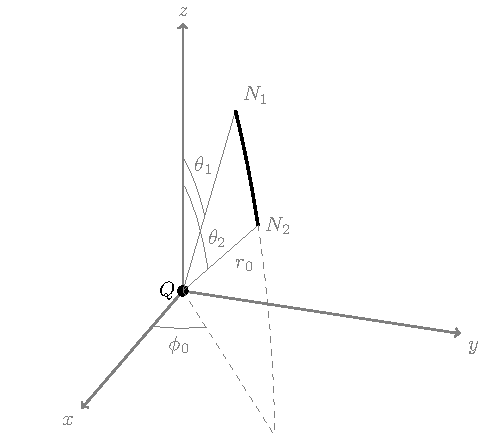
\includegraphics{figEnergyLineIntegralAlongTheta}
\caption{نقطہ چارج کے گرد صرف \عددیء{\theta} تبدیل کرتے ہوئے حرکت کا راستہ}
\label{شکل_توانائی_نقطہ_چارج_کے_گرد_تھیٹا_تبدیل_کرتے_راستہ}
\end{figure}

تصور کریں کہ \عددیء{\phi=\phi_0} اور \عددیء{r=r_0} رکھتے ہوئے ہم \عددیء{\theta} کو \عددیء{\theta_1} تا \عددیء{\theta_2} ریڈیئن  تبدیل کرتے ہوئے  چارج کو نقطہ \عددیء{N_1} سے  \عددیء{N_2} تک حرکت دیتے ہیں۔یہ صورت حال شکل \حوالہ{شکل_توانائی_نقطہ_چارج_کے_گرد_تھیٹا_تبدیل_کرتے_راستہ} میں دکھائی گئی ہے۔کروی محدد استعمال کرتے ہوئے
\begin{align*}
\dif \kvec{L}=\dif r \ar+ r \dif \theta \atheta+r \sin \theta \dif \phi \aphi
\end{align*} 
لکھا جاتا ہے۔یوں درکار توانائی
\begin{align*}
W&=-q\int_{\textup{ابتدا}}^{\textup{اختتام}} \kvec{E} \cdot \dif \kvec{L}\\
&=-q \int_{r_0, \theta_1,\phi_0}^{r_0,\theta_2,\phi_0}\frac{Q}{4 \pi \epsilon_0 r^2} \ar \cdot (\dif r \ar+ r \dif \theta \atheta+r \sin \theta \dif \phi \aphi)\\
&=-q \int_{r_0}^{r_0}\frac{ Q \dif r}{4 \pi \epsilon_0 r^2}\\
&=0
\end{align*}
صفر ہی حاصل ہوتی ہے۔یہاں دوسرے قدم پر \عددیء{\ar \cdot \ar=1} کے علاوہ \عددیء{\ar \cdot \atheta=0} اور \عددیء{\ar \cdot \aphi=0} کا استعمال کیا گیا۔

اس کے برعکس اگر نقطہ \عددیء{(r_1,\theta_1,\phi_1)} تا نقطہ \عددیء{(r_2,\theta_2,\phi_2)} چارج کو حرکت دی جائے تب
\begin{align*}
W&=-q \int_{r_1, \theta_1,\phi_1}^{r_2,\theta_2,\phi_2}\frac{Q}{4 \pi \epsilon_0 r^2} \ar \cdot (\dif r \ar+ r \dif \theta \atheta+r \sin \theta \dif \phi \aphi)\\
&=-q \int_{r_1}^{r_2}\frac{ Q \dif r}{4 \pi \epsilon_0 r^2}\\
&=\frac{qQ}{4 \pi \epsilon_0} \left(\frac{1}{r_2}-\frac{1}{r_1} \right)
\end{align*}
ہو گا۔ یوں \عددیء{r_1 > r_2} کی صورت میں جواب مثبت ہو گا اور چارج کو ابتدائی نقطے سے اختتامی نقطے منتقل کرنے کے خاطر بیرونی توانائی درکار ہو گی جبکہ \عددیء{r_2>r_1} کی صورت میں جواب منفی حاصل ہوتا ہے لہٰذا چارج کے حرکت سے ہمیں توانائی حاصل ہو گی۔
%=====
\ابتدا{مشق}
میدان \عددیء{\kvec{E}=3x^2yz^2 \ax+x^3z^2\ay+2x^3yz\az \, \si{\volt \per \meter}} میں محدد کے مرکز \عددیء{(0,0,0)} سے نقطہ \عددیء{(2,3,5)} تک دو کولمب کا چارج مندرجہ ذیل راستوں منتقل کرنے کے لئے درکار توانائی حاصل کریں۔

\begin{itemize}
\item
دو نقطوں کے مابین سیدھی لکیر۔
\item
ایسا راستہ جس پر \عددیء{y=\tfrac{3}{4}x^2} اور \عددیء{z=\frac{x}{2}+x^2} ہوں۔
\end{itemize}

جوابات: سیدھی لکیر پر \عددیء{y=\tfrac{3}{2}x} اور \عددیء{z=\tfrac{5}{2}x} لکھا جائے گا۔جوابات کے مطابق توانائی درکار نہیں بلکہ حاصل ہو گی۔\عددیء{\SI{-1200}{\joule}}، \عددیء{\SI{-1200}{\joule}} 
\انتہا{مشق}
%============
\حصہ{برقی دباو}
چارج \عددیء{q} کے منتقلی کے لئے درکار  توانائی سے زیادہ اہم  اکائی چارج کے منتقلی کے لئے درکار توانائی ہے۔اس توانائی کو \اصطلاح{برقی دباو}\فرہنگ{برقی دباو}\حاشیہب{voltage}\فرہنگ{voltage} کہتے  ہیں۔برقی دباو کے اکائی \عددیء{\si{\joule / \coulomb}} کو \اصطلاح{وولٹ}\فرہنگ{وولٹ}\حاشیہب{volt}\فرہنگ{volt} کا نام دیا گیا ہے جسے \عددیء{\si{\volt}} سے ظاہر کیا جاتا ہے۔چونکہ توانائی غیر سمتی یعنی مقداری ہے لہٰذا برقی دباو بھی مقداری ہے۔مساوات \حوالہ{مساوات_دباو_لکیری_تکملہ} سے برقی دباو یوں حاصل ہوتا ہے
\begin{align}
V_{AB}=\frac{W}{q}=-\int_{B}^{A} \kvec{E} \cdot \dif\kvec{L}
\end{align}
جہاں ابتدائی نقطے کو \عددیء{B}، اختتامی نقطے کو \عددیء{A} اور حاصل جواب کو \عددیء{V_{AB}} لکھا گیا ہے۔\عددیء{V_{AB}} لکھتے ہوئے زیر نوشت میں پہلے اختتامی نقطہ  \عددیء{A} اور بعد میں ابتدائی نقطہ \عددیء{B} لکھا گیا ہے۔عموماً برقی دباو کے مسائل حل کرتے ہوئے ابتدائی نقطے کو لامحدود فاصلے پر تصر کرتے ہوئے حاصل جواب کو \عددیء{V_A} لکھا جاتا ہے جہاں صرف اختتامی نقطے کو جواب میں ظاہر کیا گیا ہے۔ہمارے ملک میں \عددیء{\SI{220}{\volt}} برقی دباو مہیا کی جاتی ہے۔یوں منفی تار سے مثبت تار تک \عددیء{\SI{1}{\coulomb}} کا چارج منتقل کرنے کی خاطر \عددیء{\SI{220}{\joule}} توانائی درکار ہو گی۔
%==============================

